\DocumentMetadata{
  pdfversion=2.0,
  lang=es-MX,
  pdfstandard=ua-2
}

\documentclass{sener2025}

\title{Test Figuras}
\author{Test}
\date{\today}
\setDocumentoCorto{TestFiguras}

\begin{document}

\section{Figura sin centering explícito}

\begin{figure}[H]
  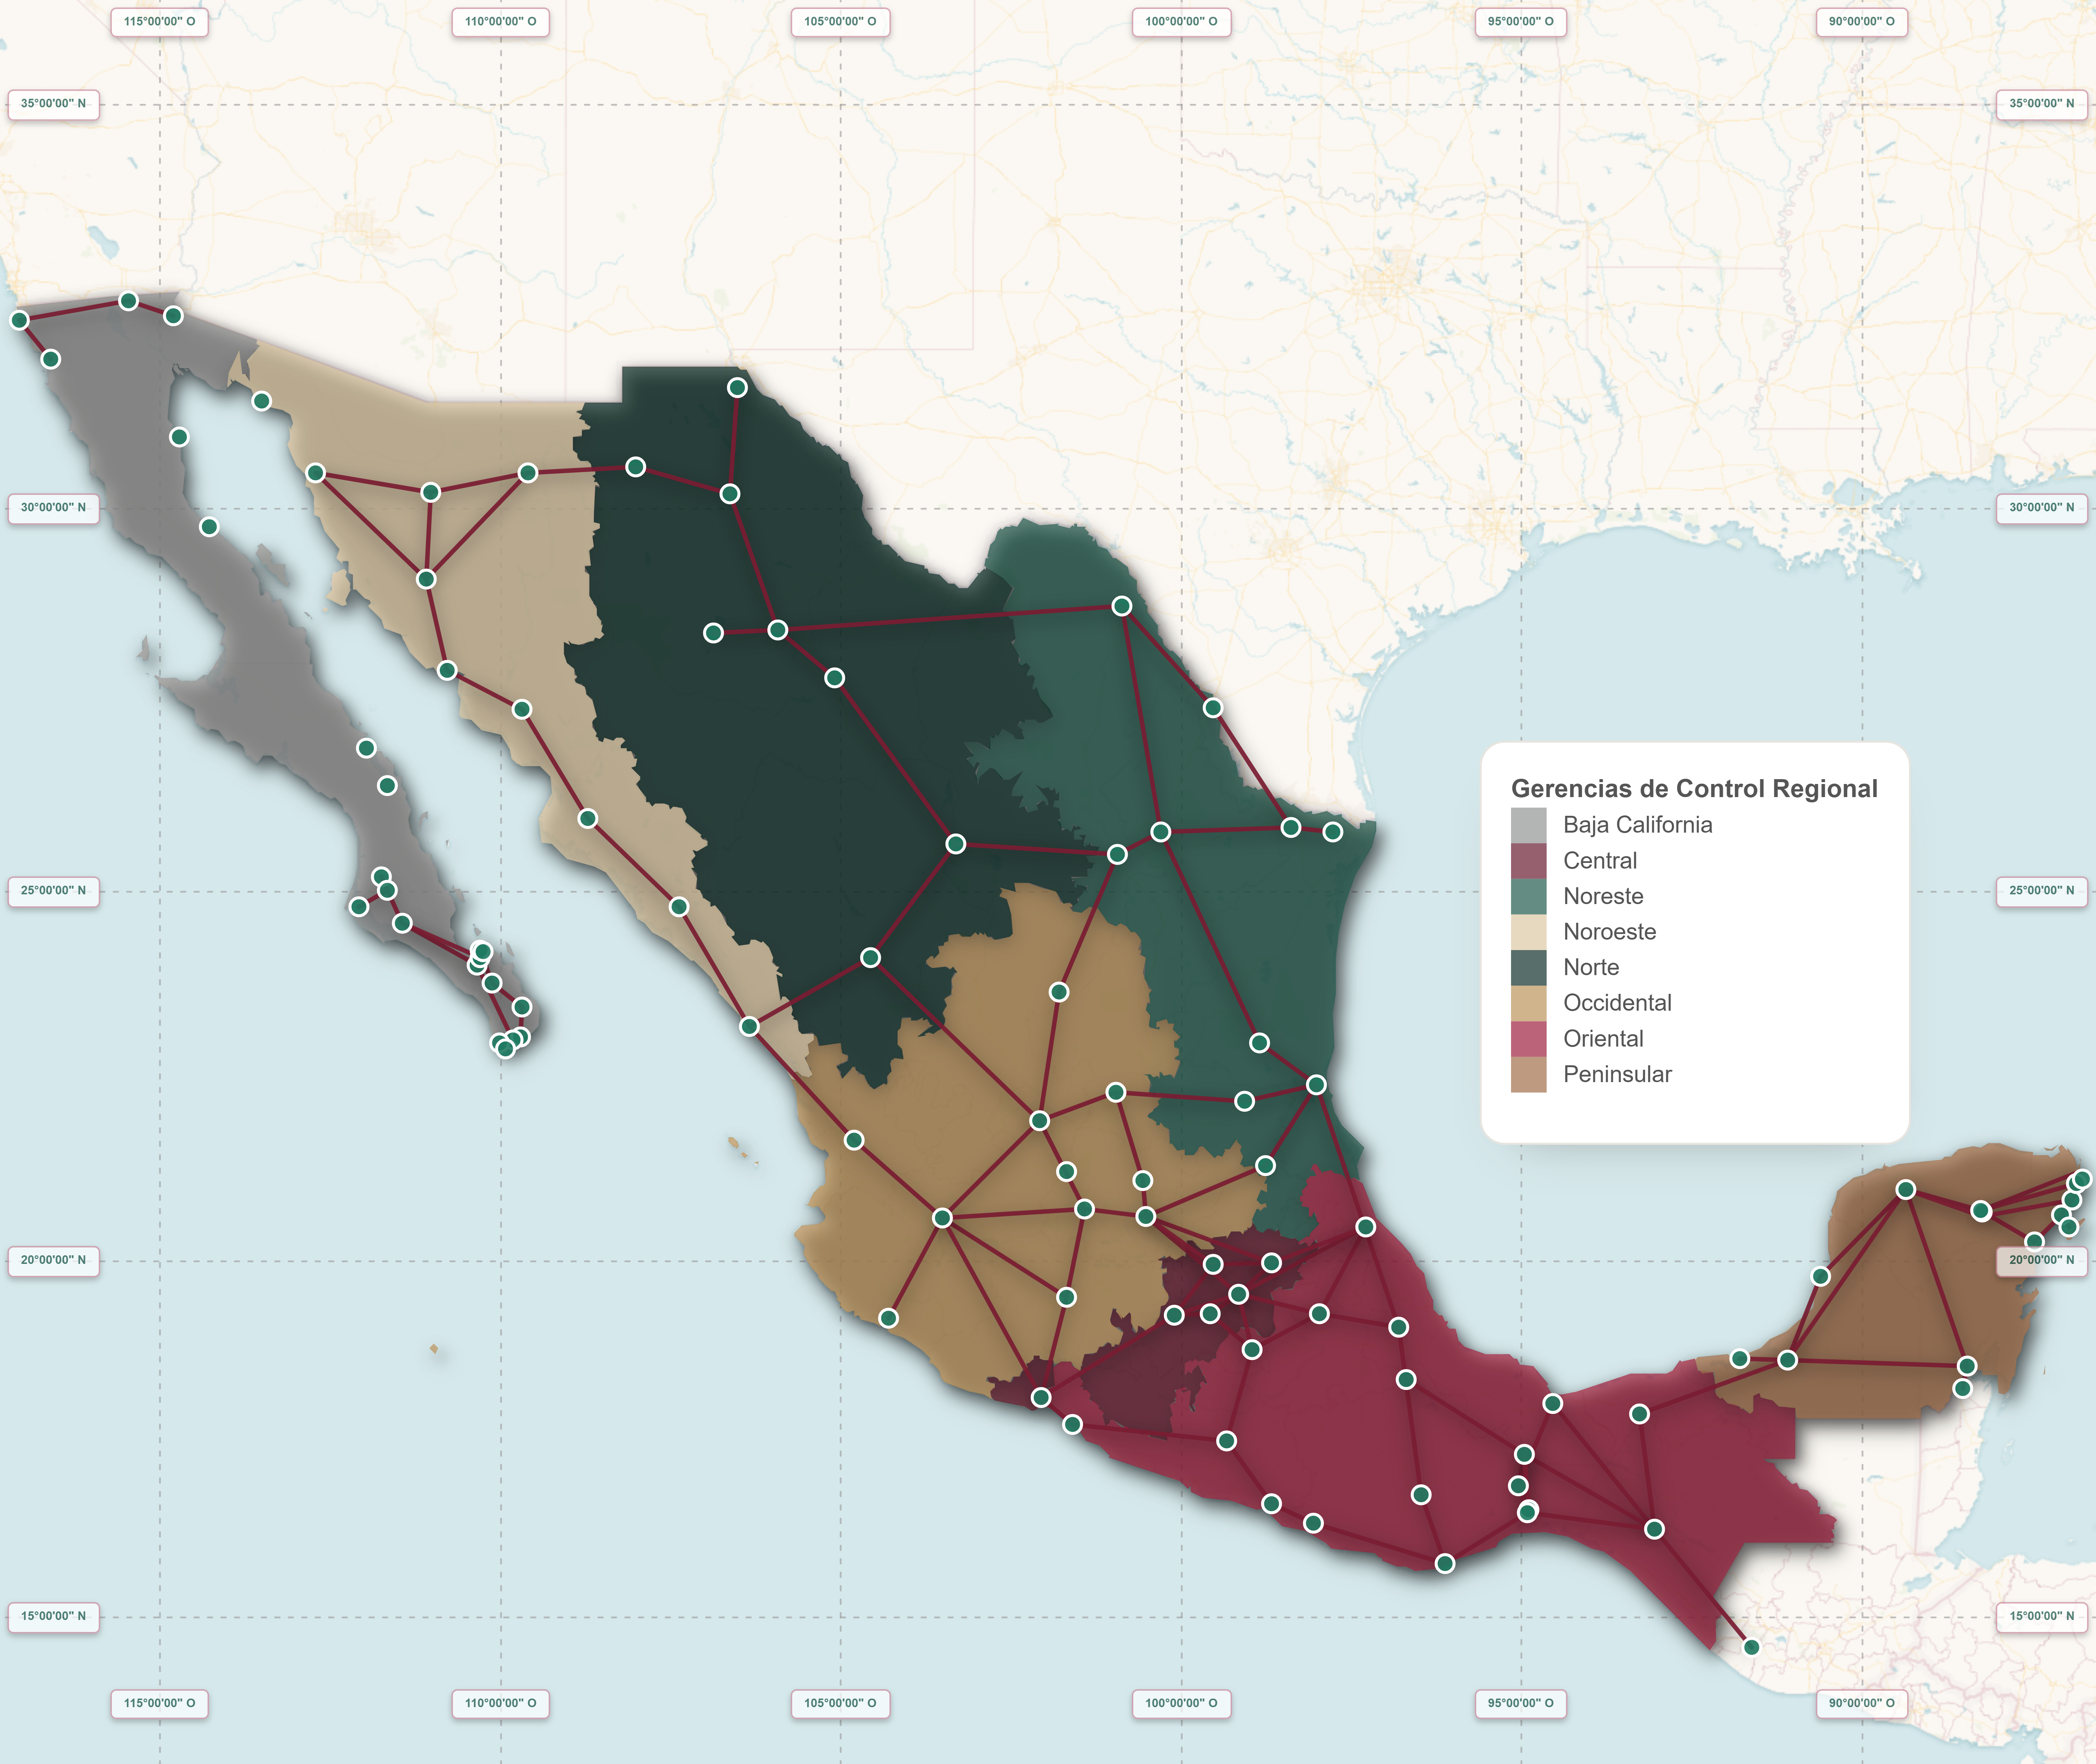
\includegraphics[width=0.8\textwidth]{img/graficos/figura_2_1.png}
  \caption{Caption corto: debería iniciar en el margen izquierdo del texto, NO centrado bajo la imagen}
  \label{fig:test-a}
\end{figure}

\section{Figura con {\textbackslash centering ...} como en Informe}

\begin{figure}[H]
  {\centering
  \pdftooltip{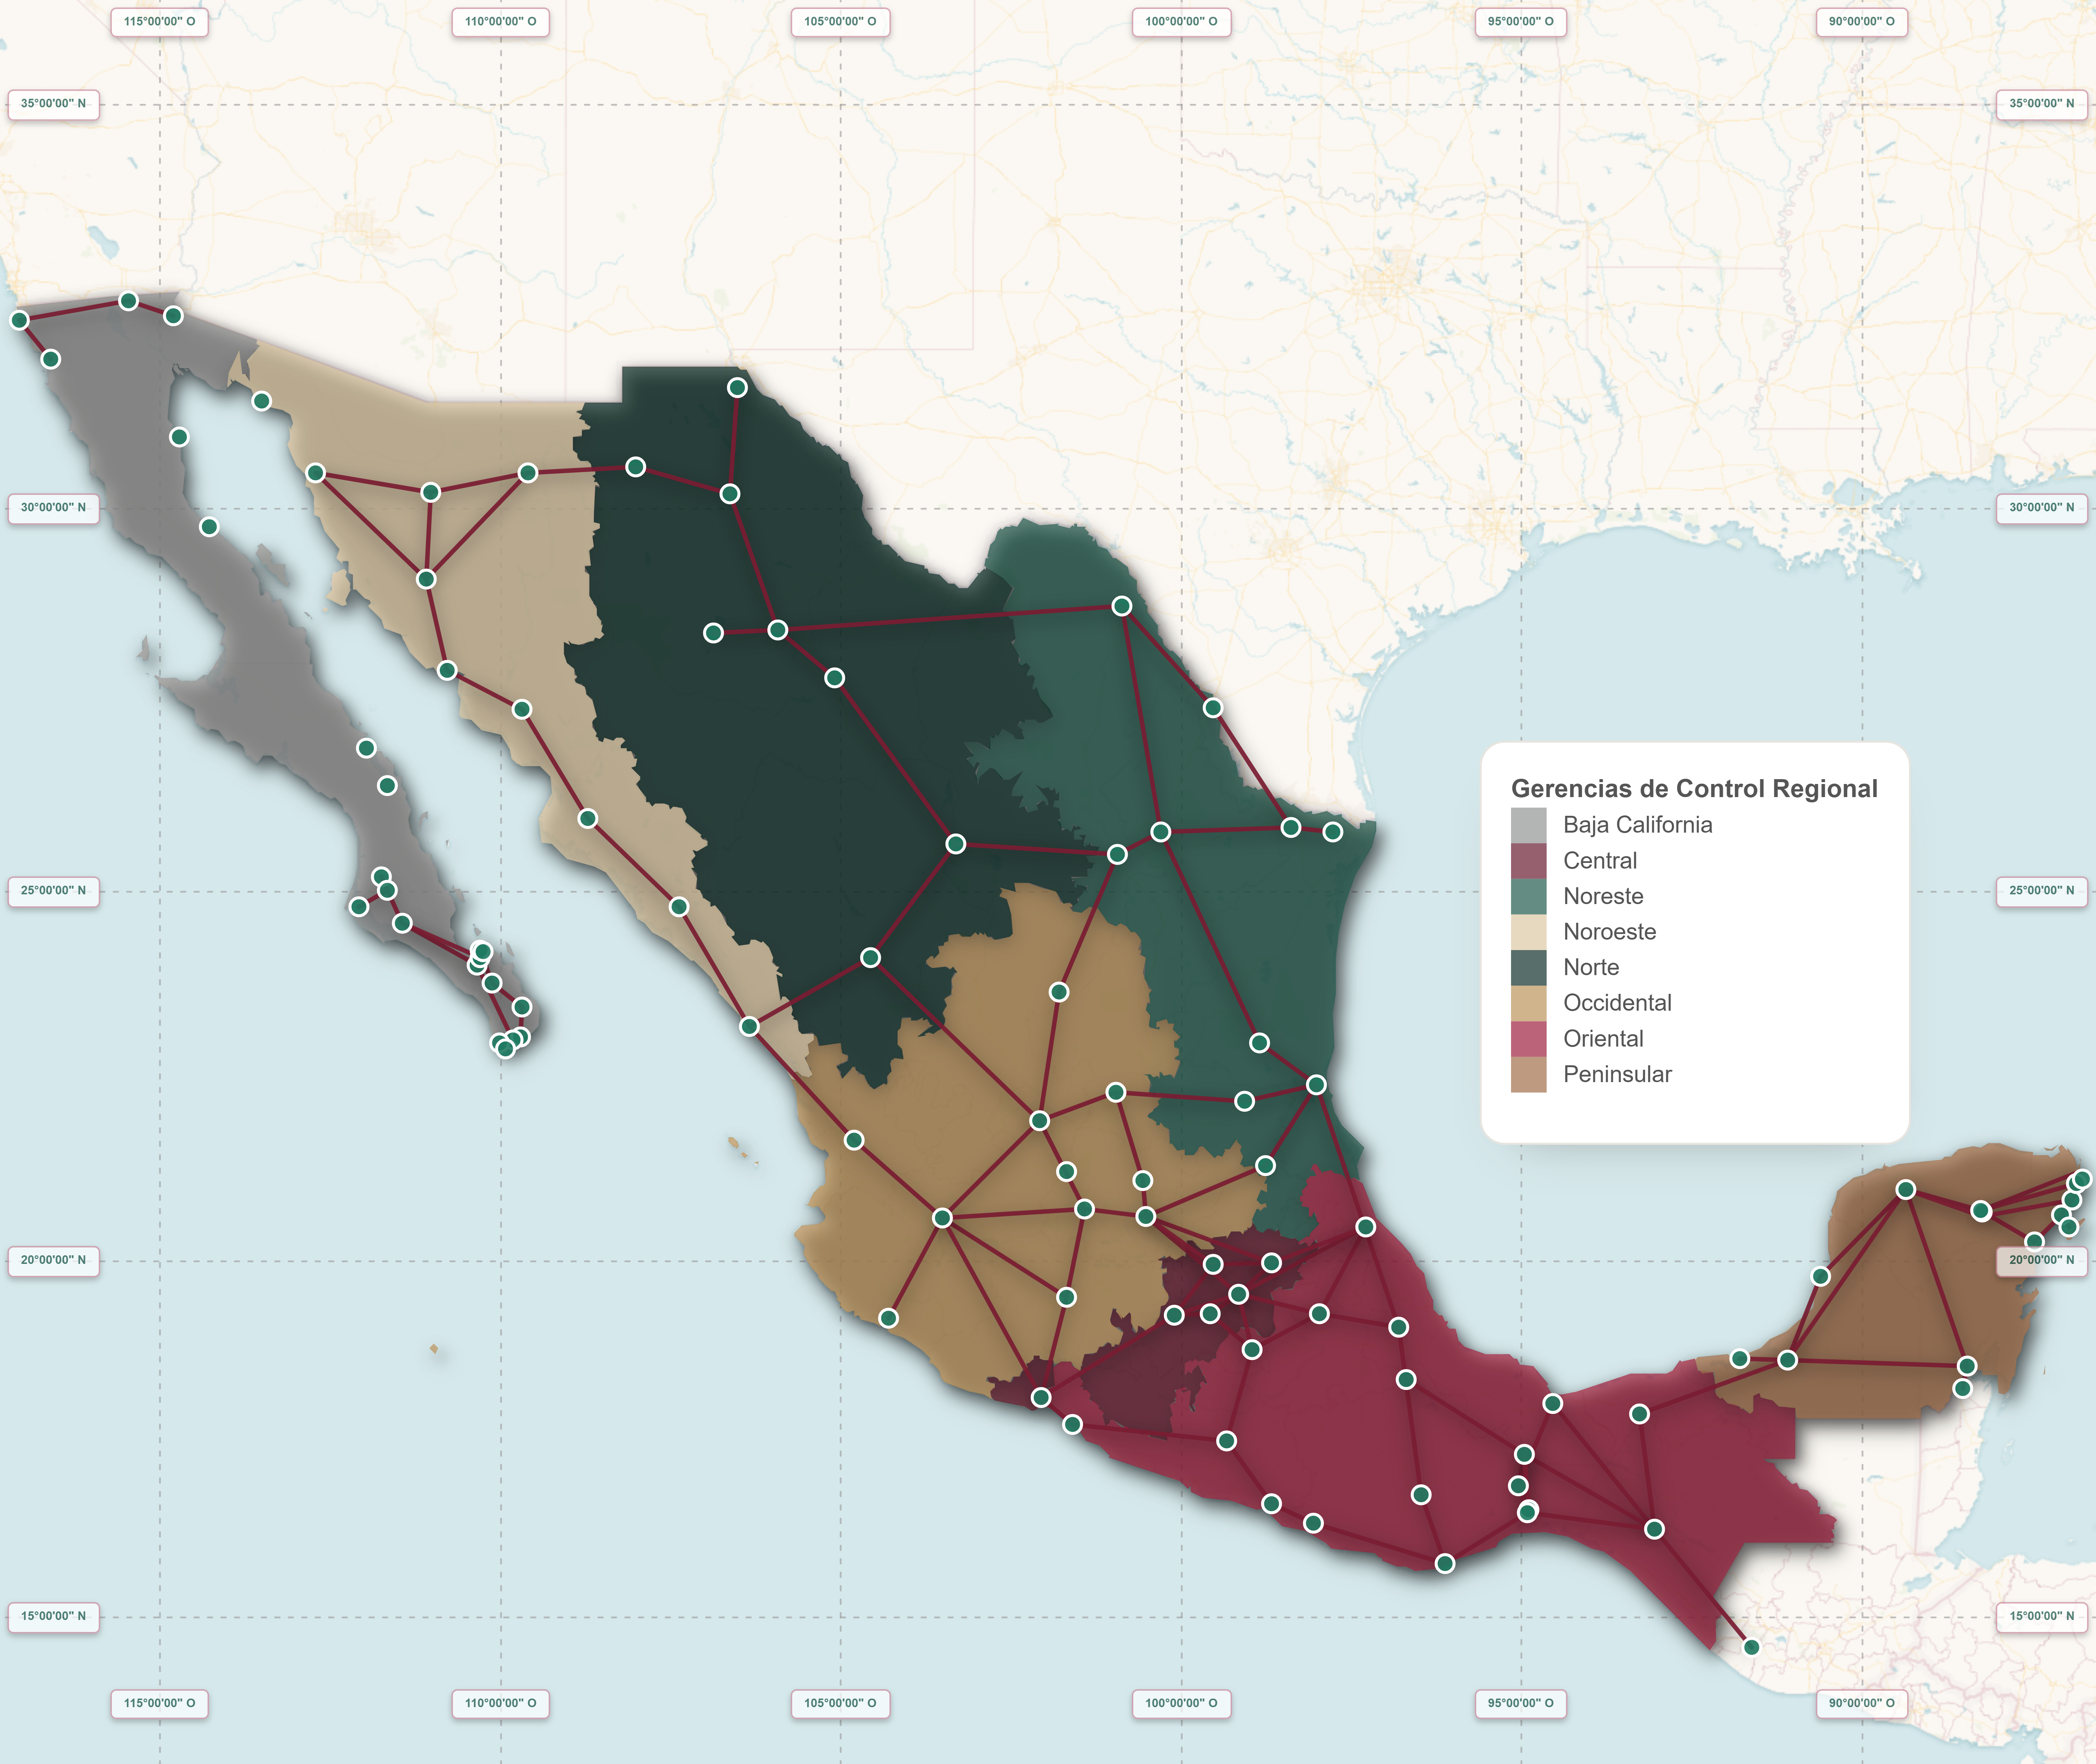
\includegraphics[width=0.8\textwidth]{img/graficos/figura_2_1.png}}{Imagen de prueba para validar captions.}
  \par}
  \raggedright
  \caption{Caption corto: debería iniciar en el margen izquierdo del texto, NO centrado bajo la imagen}
  \label{fig:test-b}
\end{figure}

\section{Figura con caption largo (multilínea)}

\begin{figure}[H]
  {\centering
  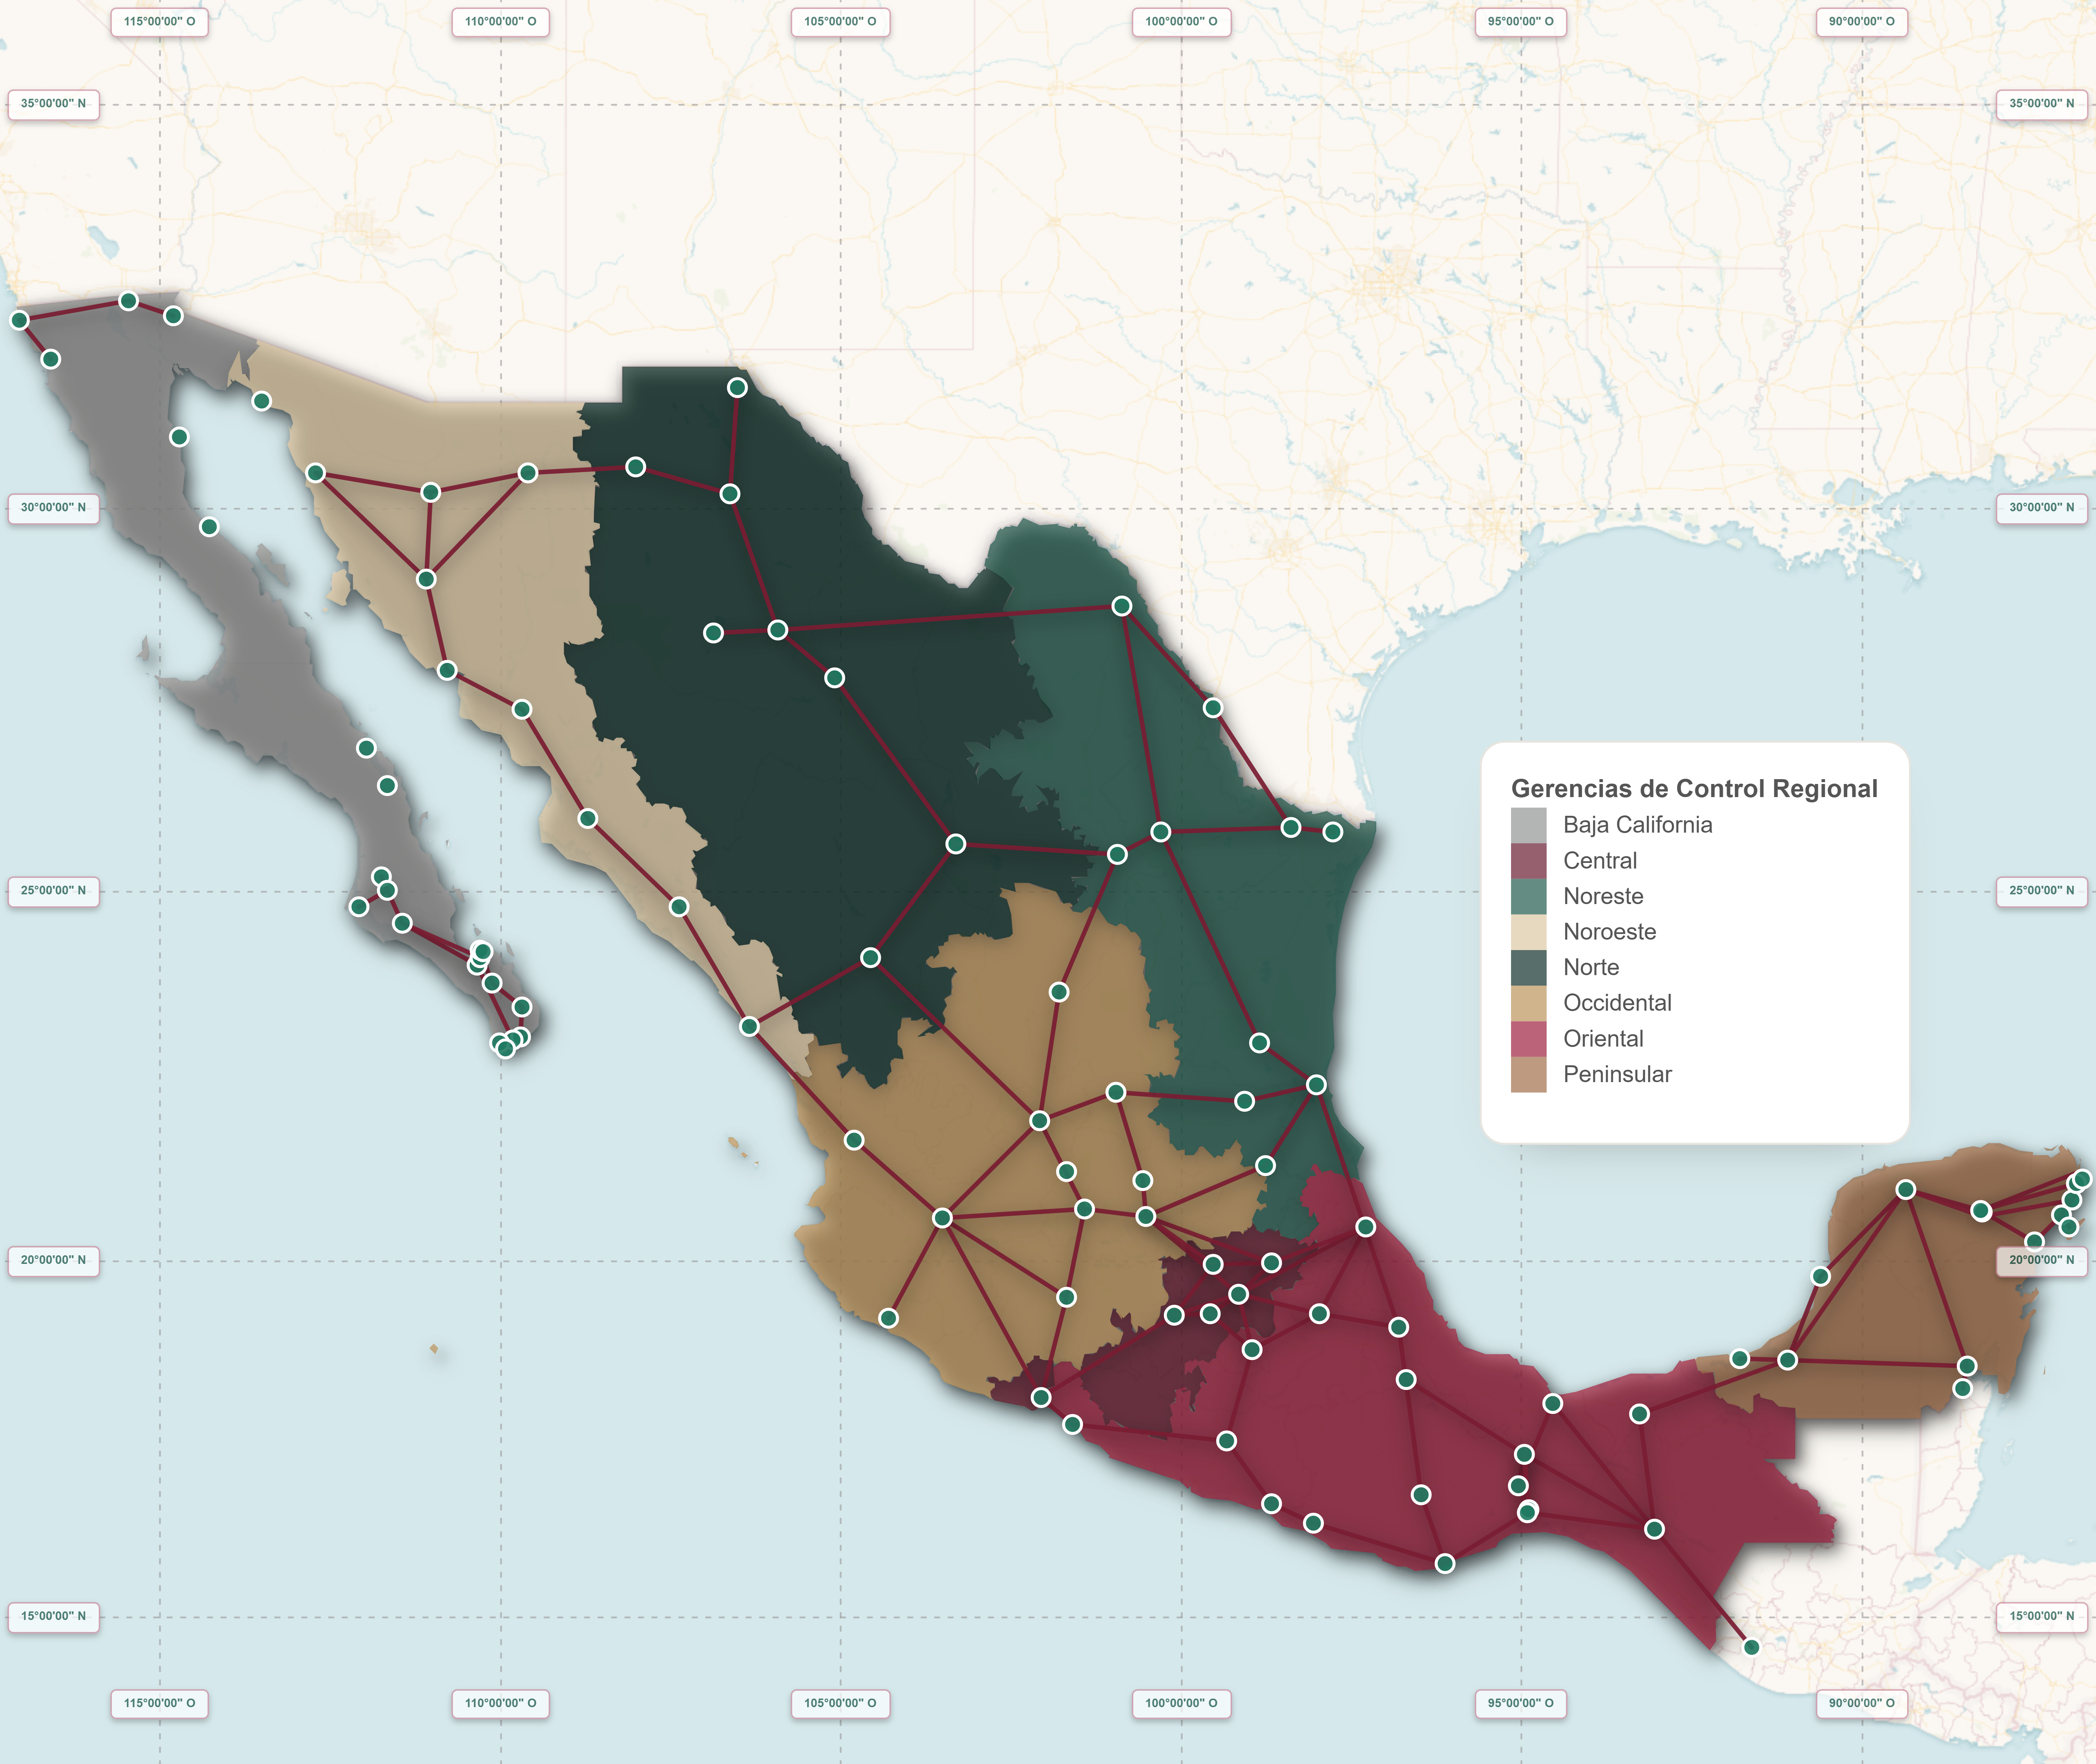
\includegraphics[width=0.8\textwidth]{img/graficos/figura_2_1.png}
  \par}
  \raggedright
  \caption{Caption largo: esta línea es deliberadamente extensa para forzar un salto y verificar que el bloque del caption sea de ancho completo y quede alineado a la izquierda del margen del texto, con el resto de líneas también en raggedright.}
  \label{fig:test-c}
\end{figure}

\end{document}
